\section{Building blocks}

%\frame {
%  \frametitle{Technological bricks and mortar}
%  \begin{itemize}
%    \item Code generation entails a tuple $<Source, Target>$
%    \item Source is the Architecture Analysis \& Design Language
%    \item Target language is Ada Ravenscar Profile
%    \item Runtime is the Open Ravenscar Kernel (ORK)
%    \item AADL \& Ravenscar Profile are key technologies
%  \end{itemize}
%}

\subsection[AADL]{Architecture Analysis \& Design Language}
\frame {
  \frametitle{AADL---The background}
  \begin{itemize}
    \item An ADL descendant of MetaH from Honeywell
    \item Major industrial entities are involved
    \item Allows modeling of runtime entities
      \pause
    \item Via components with well-defined interfaces
      \pause
    \item Which are connected together, giving communication toplogy
      \pause
    \item Different \emph{categories} of components
      {\footnotesize
        \begin{tabular}{|l|l|l|}
          \hline
          \textbf{Software} & \textbf{Hardware} & \textbf{Hybrid}\\
          \hline
          Process & Processor & System\\
          Thread & Device & \\
          Thread group & Bus & \\
          Data & Memory & \\
          Subprogram & & \\
          \hline
        \end{tabular}
      }
      \pause
    \item Separation of component interfaces \& implementations
  \end{itemize}
}

\frame {
  \frametitle{AADL---So what can I do with it?}
  \begin{itemize}
    \item Arch. description of apps, using constructs like processes,
      threads, processors etc.
    \item Only \alert{non-functional} aspects can be described
    \item Functional aspects (behavior) defined separately
  \end{itemize}
  \pause
  \begin{center}
    $\includegraphics[scale=0.5]{../figs/comp_code}$
  \end{center}
}

\frame {
  \frametitle{AADL---Component features and properties}
  \begin{itemize}
    \item \alert{Feature} is an interface point on a component
    \item Ports, subprograms, data accesses, subprogram accesses and
      parameters
    \item Features are connected together
      \pause
    \item \alert{Properties} are $<Name, Value>$ pairs attached to
      components
    \item Describe aspects not otherwise expressible
    \item Attached to types, implementations and instances
    \item E.g., \texttt{Dispatch\_Protocol}, \texttt{Period} for
      threads
  \end{itemize}
}

\subsection{Ada Ravenscar Profile}

\frame {
  \frametitle{Ravenscar---High-integrity Profile for Ada}
  \begin{itemize}
    \item The Ada language is rich in tasking constructs
    \item Tasks, and protected objects to let them interact
    \item Rendezvous among tasks also possible
    \item Ravenscar Profile is a restriction of these rich facilities
    \item Restrictions allow \emph{a priori} feasibility analysis
    \item Allow safety property guarantees
      \begin{itemize}
        \item No deadlock
        \item Bounded priority inversion
      \end{itemize}
      \pause
    \item Good choice for hard real-time systems
    \item Sporadic tasks allows protection from \alert{event storms}
  \end{itemize}
}

\begin{comment}
\frame {
  \frametitle{Ravenscar---The Restrictions}
  \begin{itemize}
    \item No creation/destruction of tasks/protected objects
    \item No synchronous communication
    \item All communication/synchronization via protected objects
    \item All protected objects must obey priority ceiling
      protocol
    \item At most one entry per protected object
    \item Data exchange via protected objects with only procedures
    \item Event signaling via protected objects with an entry
    \item \texttt{FIFO\_Within\_Priorities} scheduler, a kind of FFPS
  \end{itemize}
}
\end{comment}

\frame[containsverbatim] {
  \frametitle{Ravenscar---Patterns}
  \emph{Profile not set of patterns, but they are useful guidelines}
       {\footnotesize
         \begin{center}
           \begin{lstlisting}[language=ada,size=\tiny]
task Sporadic is
  Min_Separation : Time_Span;
  Next_Dispatch : Time;
begin
  Min_Separation := Min_Separation_P;
  loop
    Event_Object.Await;
    Next_Dispatch := Clock + Min_Separation;
    -- ... Non-suspending sporadic response code ...
    delay until Next_Dispatch;
  end loop;
end Sporadic;
           \end{lstlisting}
         \end{center}
       }
}

